\documentclass[12pt, a4paper]{article}

%%
% PREAMBLE
%%

\usepackage{geometry}   % Edit document margins
\usepackage{hyperref}   % Table of contents hyperlinks
\usepackage{parskip}    % Paragraph indent & skip
\usepackage{graphicx}   % 'graphics' package interface
\usepackage{colortbl}	% Colored tables
\usepackage{listings}   % Code sections formatting
\usepackage{xcolor}     % More colors
\usepackage{amsmath}    % Math
\usepackage{amsfonts}   % Math fonts
\usepackage{amssymb}    % Math symbols
\usepackage{blindtext}  % Placeholder text
\usepackage{setspace}   % Iterline spacing
\usepackage{multicol}   % Multicolumns
\usepackage{wrapfig}    % Figure wrapping
\usepackage{caption}    % Captions
\usepackage{tikz}       % Charts
\usepackage{makecell}   % Helper for flowcharts

% Tikz imports and setup for flowcharts
\usetikzlibrary{shapes.geometric, arrows}
\tikzstyle{block} = [rectangle, rounded corners, minimum width=1.7cm, minimum height=0.5cm,text centered, draw=black]
\tikzstyle{arrow} = [thick,->,>=stealth]

% Image caption setup
\captionsetup{labelformat=empty}

% Custom Colors
\definecolor{AnnotationGreen}{RGB}{34, 128, 45}
\definecolor{CommentGreen}{RGB}{29, 204, 49}

% Hyperlink setup
\hypersetup{
    colorlinks,
    citecolor = blue,
    filecolor = blue,
    linkcolor = blue,
    urlcolor = blue
}

% Python code formatting
% Use it by creating an environment like \begin{lstlisting}[style=Python] ... \end{lstlisting}
% Since annotations aren't tagged as keywords I have inserted a manual delimiter for them,
% it works as follows: \@@AnnotationText@@/
\lstdefinestyle{Python}{
    language = Python,
    basicstyle = \footnotesize\ttfamily,
    commentstyle = \textcolor{CommentGreen},
    stringstyle = \textcolor{orange},
    showstringspaces = false,
    keywordstyle = \textcolor{blue},
    moredelim = [is][\textcolor{AnnotationGreen}]{\\@}{@@\/},   % Annotations
    numberstyle = \scriptsize\ttfamily\textcolor{gray},
    numbers = left,
    frame = single,
    frameround = tttt,
    framexleftmargin = 20pt,
    framexrightmargin = 20pt
}

%%
% DOCUMENT
%%

\begin{document}

% Title
%---------------------------------------------------------------------
%   TITLE
%---------------------------------------------------------------------

% Margins for the title
\newgeometry{top=7cm, bottom=2cm} 

\begin{titlepage}
    \centering
    \vspace{1em}
    
    % Main title
    {\Huge\bfseries CLIP Hackathon Task \\ \normalsize\bfseries Advanced Topics in Deep Learning: The Rise of Transformers}
    
    \vspace{4em}
    
    % Professor
    {\large\scshape Prof.~Matteo Matteucci\par} 
    
    \vspace{3em}
    
    % Date
    {\large\slshape December 2023 \par}
    
    \vspace{3em}
    
    % Authors
    \begin{multicols}{2}
        \large\itshape
        Raul Singh 
        \vfill\null\columnbreak
        Davide Rigamonti
    \end{multicols}
    
    \vfill
    
    % Polimi logo
    \begin{figure}[b]
        \includegraphics[scale=0.6]{img/polimi.png} 
        \centering
    \end{figure}
\end{titlepage}

\newpage

% ToC
{
    \hypersetup{hidelinks}
    \tableofcontents
}

\pagenumbering{gobble}
\newpage
\pagenumbering{arabic}

% Margins
\newgeometry{top=1cm,left=1.5cm,right=1.5cm,bottom=2cm}

% Introduction
\section{Introduction}
This is a project that has been developed in the context of the \textit{Advanced Topics in Deep Learning: The Rise of Transformers} course held at \textit{Politecnico di Milano} and supervised by Professor Matteo Matteucci.
The initial assignment was carried out as a one-day hackathon held at Politecnico on the 1st of February 2023.
Then, groups composed of M.Sc.\ students were asked to improve upon their initial design in order to overtake their baseline performance by means of creative additions and overall improvements.

Groups were expected to implement their designs from scratch, without copy-pasting pieces of code from the assigned references.
The language recommended for the implementation is \href{https://www.python.org/}{Python}, with the addition of the \href{https://www.tensorflow.org/}{TensorFlow}/\href{https://keras.io/}{Keras} libraries.

We used \href{https://jupyter.org/}{Jupyter Notebooks} as a way to organize our work into self-contained and meaningful subtasks, we utilized \href{https://www.kaggle.com/}{Kaggle} and \href{https://colab.research.google.com}{Google Colab} as means to access computing power to train our models when local resources weren't available to us and lastly, we chose \LaTeX~to write the final report.

\subsection{Task}
The central challenge for this project is to develop a functional implementation of the \href{https://openai.com/}{OpenAI} \textbf{CLIP} model for the main task of \textbf{image retrieval} in a biomedical application.
The following \href{https://openai.com/research/clip}{blog post} and \href{https://arxiv.org/pdf/2103.00020.pdf}{research paper} were given in the assignment as a starting point for understanding the principles of the model, in addition to the information already given by Professor Giacomo Boracchi during the course frontal lectures.

\subsubsection*{CLIP Principles}
In short, \textbf{CLIP} stands for \textbf{C}ontrastive \textbf{L}anguage-\textbf{I}mage \textbf{P}re-training, and it is composed by two \textit{encoders} (one dedicated to images and one for text) which are trained to minimize the loss computed as the \textit{cosine similarity} of the embedded image pairs.

This peculiar pre-training technique enables the model to achieve relevant performance metrics on a wide array of zero-shot tasks (such as classification) while using a fraction of the dataset of other popular deep learning models performing the same task.

\subsection{Dataset Analysis}

The dataset provided is a \textit{simplified} version of the \href{https://link.springer.com/chapter/10.1007/978-3-030-01364-6_20}{\textbf{ROCO} dataset} (\textbf{R}adiology \textbf{O}bjects in \textbf{CO}ntext) which consists of \textit{83275} elements composed of:

\begin{itemize}
    \item A low resolution image that has been reduced in size.
    \item A corresponding textual caption that describes the image.
    \item A set of concept labels that characterizes the attributes of the image.
\end{itemize}

There are \textit{80813} unique captions as most of them are present in the database only one time, the most common caption appears in \textit{261} images.

Images can have from \textit{1} to \textit{50} concepts associated to them from a total of \textit{8374} concepts, averaging around \textit{5} concepts per image.

Concepts can have from \textit{2} to \textit{25989} images associated to them from a total of \textit{83275} concepts, averaging around \textit{47} images per concept.


\begin{figure}
        \hspace*{-4.5em}
        \begin{minipage}{25em}
            \centering
            \includegraphics[width=22em]{img/Data_Exploration_2.png}
            \caption{Concepts per Image}
        \end{minipage}
        \begin{minipage}{25em}
            \centering
            \includegraphics[width=25em]{img/Data_Exploration_3.png}
            \caption{Images per Concept}
        \end{minipage}
\end{figure}


% Hackathon Results
\section{Hackathon Results}
The self-imposed goal for the hackathon was to build a CLIP model capable of performing image retrieval, thus we initially left out the portion of data regarding concepts and labels.

Unfortunately we didn't manage to create a functioning notebook in the allotted time.
However, we can still consider ourselves satisfied with our work, since right after the event we noticed that we were just a small change away to obtain a fully working CLIP model.

\subsection{Initial Intuition}
During the hackathon, we opted for splitting our efforts into two separate tasks: model creation and data gathering.
We created 2 preliminary notebooks that tackled the defined tasks, these notebooks were then joined together into a single notebook, considered the final product for the hackathon.

\subsubsection{Data Gathering}
Since the given dataset was problematic to handle due to its dimension and its uncommon compression encoding, part of our efforts were dedicated to create a proper \textit{data pipeline} to feed the model.

The preliminary data gathering pipeline loads captions and images separately, performing different preprocessing for both of them (using the \textit{transformer custom standardization function} seen during lectures for textual data, while performing \textit{resizing} and \textit{normalization} for image pixel data).
The captions are then vectorized using a \href{https://www.tensorflow.org/api_docs/python/tf/keras/layers/TextVectorization}{Keras text vectorization layer}, all the elements are split manually into train, test and validation sets and stored into Python lists.

Various visualizations of the imported images and data were added to ensure the correctness of the loading process.

\subsubsection{Model Creation}
For the preliminary model we decide to implement the encoders from scratch in order to avoid adding useless complexity to our prototype.

For the image encoding we defined a simple CNN composed by 3 \href{https://www.tensorflow.org/api_docs/python/tf/keras/layers/Conv2D}{convolutional layers} with increasing neuron count (from 64 to 256 neurons) with the inclusion of \href{https://www.tensorflow.org/api_docs/python/tf/keras/layers/BatchNormalization}{batch normalization layers}.
At the top of the convolutional section we added a \href{https://www.tensorflow.org/api_docs/python/tf/keras/layers/Flatten}{flattening layer} followed by two \href{https://www.tensorflow.org/api_docs/python/tf/keras/layers/Dense}{dense layers} to obtain a final embedding of size 128.
All of the hidden layers have \href{https://www.tensorflow.org/api_docs/python/tf/keras/layers/ReLU}{ReLU} activation functions.

% TODO: check positional embedding method
For the text encoding we used a \textit{transformer encoder block} that was presented during the course lectures, which makes use of \href{https://www.tensorflow.org/api_docs/python/tf/keras/layers/MultiHeadAttention}{multi-head attention}, \href{https://www.tensorflow.org/api_docs/python/tf/keras/layers/LayerNormalization}{layer normalization} and \href{https://www.tensorflow.org/api_docs/python/tf/keras/layers/Dropout}{dropout} layers; at the end of the block there are 2 \textit{dense layers} to obtain a final embedding of size 128.
Before being fed to the encoder block, inputs pass through a double \href{https://www.tensorflow.org/api_docs/python/tf/keras/layers/Embedding}{embedding layer} that implements \textit{positional embedding} by addition.

The complete model routes the two inputs (image and text) to their respective encoders, normalizes the resulting embeddings and obtains the \textit{logits} by applying the formula outlined in the OpenAI paper: $logits = (I_e \cdot T_e^{\top})e^t$.
Then, the individual losses are calculated by means of \href{https://www.tensorflow.org/api_docs/python/tf/keras/losses/CategoricalCrossentropy}{categorical cross-entropy} and are averaged to obtain the final loss.

\subsection{Idea Refining}
As mentioned before, the very last notebook obtained at the end of the hackathon didn't work correctly as there were some small discrepancies between the sizes of the expected inputs vs.\ the actual inputs, and we were trying to apply \textit{categorical cross-entropy} utilizing numeric variables that were not \textit{one-hot encoded}.

The day after the hackathon took place we dedicated some of our time to slightly refine the final product obtained in order to have a functioning model.
By adapting the structure of our network to the input data, fixing minor conflicts related to typing and employing \href{https://www.tensorflow.org/api_docs/python/tf/keras/losses/SparseCategoricalCrossentropy}{sparse categorical cross-entropy} instead of \textit{categorical cross-entropy}, we managed to obtain a working CLIP implementation.

Due to the inefficient loading technique we weren't able to hold the entirety of the dataset and the model in memory, thus we couldn't test it properly.
However, by considering a fraction of the dataset and training the model on it for around 10 epochs, we noticed that the results were quite scarce as the loss would not get any lower after the first few epochs.
When considering a top-k image-retrieval task on the training dataset with an exact caption as a query, the target image was only occasionally present in the top-10 matched results, and never in the top-5.

The reported results of this step are based on empirical observation as we did not have a proper evaluation system for this task yet.
This is due to the fact that our main goal for the hackathon was to produce a functioning model, not evaluate its performance.

% Post-Hackathon Improvements
\section{Post-Hackathon Improvements}
This section is dedicated to exploring all the improvements (successful and non) that were performed in the months following the initial hackathon challenge.
Some of these improvements are strictly related to the model structure and performance, while others are centered around \textit{data exploration}, \textit{data gathering} and \textit{model evaluation}.

\subsection{Loss Function}
We decided to reimplement the loss function and how it is integrated inside the CLIP model from scratch as we previously made use of \href{https://www.tensorflow.org/api_docs/python/tf/keras/layers/Lambda}{TensorFlow lambda layers} to perform mathematical operations.
We noticed that these layers were causing problems in both the gradient calculation process and during import/export operations.

The approach we took for the new loss was quite radical as we decided to delve into the \href{https://www.tensorflow.org/api_docs/python/tf/keras/Model}{Keras model} by \textit{overriding} the \texttt{train\char`_step} and \texttt{text\char`_step} in order to have more control on how the model calculates loss and how it performs its backpropagation process.
Although we modified the overall structure of the model, the mathematical essence of the loss function remains the same as the one defined in the reference OpenAI paper.

\subsection{Lazy Loading}
It was previously mentioned that the size of the complete dataset was a critical factor that needed to be taken into account at some point.

By implementing a \textit{lazy loading} interface utilizing the \href{https://www.tensorflow.org/api_docs/python/tf/data/Dataset}{TensorFlow dataset class} and exploiting the \textit{map/reduce paradigm} with \textit{lambda functions} we were able to load the actual pixel data of images from their image path only when needed.
We wrapped this operation inside a custom function called \texttt{create\char`_dataset} that exposes a general interface which allows for parametrization of the dataset creation procedure through parameters that influence \textit{batching}, \textit{shuffling}, \textit{dataset structure}, \textit{caching} and other aspects.

At this point we noticed that the vectorization for the captions was causing a minor \textit{data leakage} from the test set to the train set, we corrected the mistake and implemented a new splitting function by wrapping the \href{https://scikit-learn.org/stable/modules/generated/sklearn.model_selection.train_test_split.html}{scikit-learn train\_test\_split function} inside a custom function to also manage validation splits.

\subsection{Pre-Trained Models}
As previously explained, our implementation of the model was completely from scratch. At this point we encountered a performance bottleneck, impeding any further enhancement of the model. This was probably due to the huge amount of parameters in the model, which were quite a challenging task to train from scratch, even considering our large dataset.

As shown during the course lectures, we decided to try to leverage a \textit{pre-trained} model for both our image and text encoder and perform \textit{transfer learning}.

\subsubsection{Image Encoder}
For the image encoder, we chose to utilize a \href{https://github.com/facebookresearch/ConvNeXt}{ConvNeXt} network via the \href{https://keras.io/api/applications/}{Keras Applications API}, specifically the \href{https://keras.io/api/applications/convnext/#convnexttiny-function}{ConvNeXtTiny} variant, known for its compact size yet commendable performance.
We made this selection based on two primary reasons: firstly, to opt for a reasonably sized and efficient CNN to mitigate the risk of overfitting, and secondly, due to our past projects demonstrating impressive results with this network, making it a logical starting point.

\subsubsection{Text Encoder}
As for the text encoder, we employed \href{https://huggingface.co/docs/transformers/model_doc/bert}{BERT} as our preferred \textit{text transformer}.
We initially utilized the base version of the transformer as a foundation.

Importing and integrating the model as a layer within our architecture posed a challenge, given that most methods are designed for standalone use of these models.
In the end we successfully overcame this obstacle thanks to the \href{https://www.tensorflow.org/hub}{\texttt{tensorflow\_hub}} module, importing BERT as a \href{https://www.tensorflow.org/hub/api_docs/python/hub/KerasLayer}{\texttt{KerasLayer}} and seamlessly incorporating it into our model.

\subsection{Embedding Projection}
As previously explained, our architecture comprises the following components:
\begin{itemize}
    \item an \textit{image encoder} followed by a 2-layer dense neural network
    \item a \textit{text encoder} followed by a 2-layer dense neural network
\end{itemize}
The purpose of the 2-layer dense network is to project the \textit{high-level features} extracted from the encoders into a shared embedding space.
In an effort to enhance this projection, we engaged in thorough experimentation.
After extensive tinkering, we settled on a 2-layer dense network with \textit{dropout} incorporated in the middle, along with a \textit{residual connection} linking the two dense layers, culminating in \href{https://keras.io/api/layers/normalization_layers/layer_normalization/}{layer normalization}.

We also explored various activation functions, starting with \href{https://keras.io/api/layers/activation_layers/relu/}{ReLU} and subsequently testing \href{https://www.tensorflow.org/api_docs/python/tf/keras/activations/gelu}{GELU}, \href{https://www.tensorflow.org/api_docs/python/tf/nn/silu}{SiLU}, and \href{https://www.tensorflow.org/api_docs/python/tf/nn/selu}{SELU}. Ultimately, SELU demonstrated a significant improvement, prompting us to adopt it for the projection.

Both dense layers were configured with 128 neurons, resulting in a 128-dimensional embedding space.

\begin{center}
    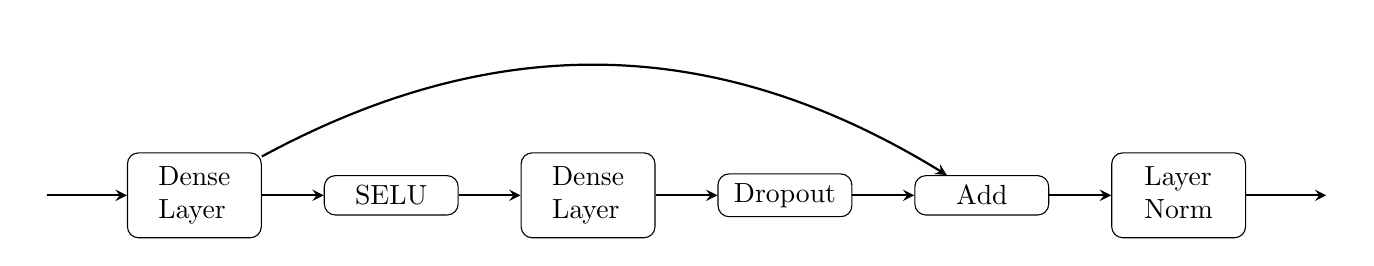
\begin{tikzpicture}[node distance=2cm]
        \node (dense1) [block] {\makecell[l]{Dense \\ Layer}};
        \node (selu) [block, right of=dense1, xshift=0.5cm] {SELU};
        \node (dense2) [block, right of=selu, xshift=0.5cm] {\makecell[l]{Dense \\ Layer}};
        \node (dropout) [block, right of=dense2, xshift=0.5cm] {Dropout};
        \node (add) [block, right of=dropout, xshift=0.5cm] {Add};
        \node (norm) [block, right of=add, xshift=0.5cm] {\makecell[l]{Layer \\ Norm}};

        \node (input) [left of=dense1] {};
        \node (output) [right of=norm] {};

        \draw [arrow] (input) -- (dense1);
        \draw [arrow] (dense1) -- (selu);
        \draw [arrow] (selu) -- (dense2);
        \draw [arrow] (dense2) -- (dropout);
        \draw [arrow] (dropout) -- (add);
        \draw [arrow] (add) -- (norm);
        \draw [arrow] (dense1) to[bend left] (add);
        \draw [arrow] (norm) -- (output);
    \end{tikzpicture}
\end{center}    

\subsection{Image Embedding}
\blindtext[1]

\subsection{Text Embedding}
\blindtext[1]

\subsection{Evaluation}
In the first steps of this project we were using the \textit{loss} returned by the model as its quality metric, which is not really optimal for various reasons, therefore we decided to write a separate notebook solely dedicated to model evaluation for the two main retrieval tasks.

The inference procedure is specular for image and text retrieval: we first generate the embeddings of the feature that we want to retrieve by calling the \texttt{predict} method of the relevant encoder on the dataset that we want to utilize.
Then, for every query of the dataset we generate the embedding through the other encoder, and we compute the \textit{cosine similarity} to then retrieve the \textit{top-k} results for each query.

Finally, we compute the mean \textbf{accuracy}, \textbf{precision}, \textbf{recall} and \textbf{F1 score} for the query dataset through \textit{micro-averaging}, and we visualize them utilizing \textit{graphs} and \textit{reports} with the possibility of comparing evaluations between models or against a random classifier baseline.
However, we noticed there are multiple \textbf{relevance metrics} that are interesting to take into consideration (explained taking into consideration image retrieval):
\begin{itemize}
    \item \textbf{Caption Equality}: a result is relevant only if its caption is equal to the original query; it can be quite restrictive since most of the captions are unique.
    \item \textbf{Concept Overlap}: a result is relevant only if it shares \textit{n} concepts with the original element; it provides a good estimate for real use-cases but can be misleading if the threshold is too low, in addition it cannot be used if the concept data is not present.
\end{itemize}

\section{Other Tasks}

\section{Results}
\blindtext[1]

\end{document}